\documentclass{report}
\usepackage[dvipsnames]{xcolor}
\usepackage[american]{babel}
\usepackage{fontspec}
\usepackage[dvipsnames]{xcolor}
\usepackage{lmodern}
\usepackage{amssymb,amsmath}
\usepackage{comment} % enables the use of multi-line comments (\ifx \fi)
\usepackage{fullpage} % changes the margin
\usepackage{todonotes}
\usepackage{graphicx}
\usepackage{import}
\usepackage{physics}
\usepackage{systeme}
\usepackage{multicol}
\usepackage{enumitem}
\usepackage[lofdepth,lotdepth]{subfig}

\usepackage[backend=biber,style=apa,url=false]{biblatex}
\addbibresource{SingingBirds.bib}
\DeclareLanguageMapping{american}{american-apa}

\usepackage{xifthen}
\usepackage{soul}
\sethlcolor{Apricot}
\newcommand\bla[1]{\ifthenelse{\isempty{#1}}{\hl{**~bla~bla~**}}{\hl{**~#1~**}}}
\usepackage[unicode=true]{hyperref}
\usepackage[all]{hypcap} % ref link to the top of the figure

\usepackage{csquotes} % Dependency for APA

\usepackage{titlesec}

\titleformat{\chapter}{\normalfont\huge}{\thechapter.}{20pt}{\Huge}


\hypersetup{breaklinks=true,
            pdfauthor={Paul Ecoffet},
            pdftitle={Master thesis Computational Model of birdsong learning},
            colorlinks=true,
            citecolor=blue,
            urlcolor=blue,
            linkcolor=black,
            pdfborder={0 0 0}
            }
\urlstyle{same} % don't use monospace font for urls


\title{Master Thesis\\ Computational model of Zebra Finch song learning and the
influence of sleep on it}
\author{Paul Ecoffet\\
Supervisors: Stéphane Doncieux, Benoît Girard}
\date{The 6th of June, 2017}

\begin{document}
\maketitle

\begin{abstract}
The Zebra Finches are songbirds which learn the song of their tutor. They learn
it from 25 days post hatch (DPH) to 90 DPH \parencite{liu_juvenile_2004}. Zebra
finches are commonly used as a model of speech acquisition.

\textcite{deregnaucourt_how_2005} showed that sleep plays an important role in
the learning of tutor songs. Indeed, they showed that sleeping has a negative
impact on song restitution by zebra finches in the short term but a positive
impact on the long run. Song restitution is less complex and less similar to the
tutor song from one morning to the previous day evening, but the greater this
loss in performance was overall for one bird, the better this bird was able to
reproduce the tutor song at the end of its learning.

In addition to that, \textcite{dave_song_2000} have found neurons in the motor
cortex which fires sequences during sleep that correspond to their activity
pattern when the birds sing in adult zebra finches. This shows that motor
neurons that are highly correlated with bird's own song (BOS) are activated
during the night. These identified replays suggest that some learning may occur
during sleep that use past experiences.

Our hypothesis is that during its sleep, the zebra finch restructures the
knowledge it has acquired so far thanks to replay mechanisms. We hypothesize
that this restructuring can account for the loss of performance in the short
term and an improvement of performance in the long term.

The goal of this internship is to offer a model of the zebra finch song
learning which can explain different behavioral data observed such as the
correlation between the loss of performance every night and the overall
performance at the end of learning.
\end{abstract}

\tableofcontents

\chapter{Introduction}\label{introduction}

\section{Zebra Finch song learning}\label{zebra-finch-song-learning}

\subsection{Characteristic of the zebra finch song
learning}\label{characteristic-of-zebra-finch-song-learning}

\todo{insert zebra finch figure}

The Zebra Finches are songbirds which learn the song of their tutor. Only males
sing. Singing is part of the courtship of the bird. They learn their tutor song
from 25 days post hatch (DPH) to 90 DPH \parencite{liu_juvenile_2004}. The songs
have rather complex structure, with a chain of syllables. A syllable is defined
by a sound surrounded by short silences. This chain of syllables forms a
``motif'' \parencite{doupe_birdsong_1999, margoliash_evaluating_2002}. Zebra
finches are close-ended learners \parencite{margoliash_sleep_2010}. They learns
only one song and will retain it their whole life, in comparison of open-ended
learners such as canaries which learns a new song each year.

The Zebra Finch learning development has been described in two different phases.
First of all, the Zebra Finch is in a sensory phase until 65DPH, when it only
listens to the song of its tutor, which can be sung by a real Zebra Finch or by
a song playback. This is a critical period in which the bird memorize fully the
tutor song. Birds who have access to the tutor song for only ten days between
25DPH and 65 DPH sing the tutor song as good as the bird with access to the
tutor song during their whole learning \parencite{bohner_early_1990,
roper_onset_2006}. The second phase is the sensorimotor phase during which the
bird sing and use its auditory feedback to improve its performance. It overlaps
the sensory phase. Starting from 25DPH to 30DPH, the bird produces a
\emph{subsong}, a process similar to babbling. Then, the bird produce a
\emph{plastic song} starting from 50DPH. It tries to imitate the tutor song it
has memorized. After 90DPH, the song has reached its \emph{crystallization}. The
song is fixed and will not change throughout the Zebra Finch adulthood. The song
of the Zebra Finch gets highly stereotyped \parencite{williams_birdsong_2004}.
Zebra Finches needs auditory feedback to learn to sing. Deafening in juvenile
has severe impact on song acquisition, even if the tutor song has already been
acquired. Deafening once the song is learned has a much smaller impact on
performance \parencite{scharff_comparative_1991, doupe_birdsong_1999}. Deafening
a chicken, in opposition, has no impact on its calls. Zebra Finches raised in
isolation will also develop abnormal songs. Therefore, Zebra Finches learns
their vocalisation from a tutor and need to hear themselves to sing correctly.

\subsection{Why is zebra finch song learning
studied}\label{why-is-zebra-finch-song-learning-studied}

Songbird and especially Zebra finches are commonly used as a comparison with
human about vocal development. Indeed, the song they produce are not innate even
though they have predispositions toward learning their songs. They produce
song with complex structures composed of syllables.

The neuroanatomy of Zebra Finch has also been extensively studied and the
different structures involved in singing has been identified
\parencite{nottebohm_neural_2005, bertram_two_2014}.
\textcite{doupe_birdsong_1999} even proposed parrallels between the areas
involved in song production with songbird and the areas involved in speech with
humans.

Zebra Finches are also excellent laboratory animals. They are easily
domesticated and easy to study compared to other songbirds or ``speaking''
animals\todo{not beautiful sentence}. As they learn only one song, their
learning is easily trackable. The developmental trajectory can be inferred.
\textcite{deregnaucourt_how_2005} for instance tracked from the syllables
trajectories by clustering syllable productions over time.

  * Well studied Neuroanatomy
  * Easy to study experimentally
        * Easily domesticated
      * Learn one song
      * Learn quickly (90DPH)
      * Easy to track song development

\section{Neurobiology of the Zebra Finch}
\label{neurobiology-of-the-zebra-finch}

\subsection{Neuroanatomy of the Zebra Finch song system}
\label{neuroanatomy-of-the-zebra-finch-song-system}

  * Connection between RA, HVC, Area X, \ldots{} Inhibition, excitation

\subsection{Pattern of activation in RA and HVC}
\label{pattern-of-activation-in-ra-and-hvc}

  * HVC clock like, temporal structure (Ali et al.)
  * RA activation while singing at very precise time and sparse coding

        * Motor control (Ali et al.) Ali et al. shows real two different
    learning: spectral and temporal

\section{Models of song learning} \label{models-of-song-learning}

Only very few models have been created. Even less are actual
computational models.

\subsection{Reinforcement learning} \label{reinforcement-learning}

  * Proposed but no real explanation of what could be the state space, the
  action space, the reward function (Dave\&Margoliash).
  * Used in paradigm to test different hypothesis (averse reward to force
  change in behaviour of the bird)

\subsection{Song preferences in selection
(Marler)} \label{song-preferences-in-selection-marler}

  * Behavioural model to explain how the bird select its template
  * TODO: Add more

\subsection{Coen's model} \label{coens-model}

  * Clustering technique with babbling (multimodal)

      * Cluster the tutor song syllables thanks to their characteristics
      * Babbling, create a mapping between the motor space and the
    identified cluster
    * Use of a real synthesizer but not actually built to model zf vocal
  apparatus
  * No quantitative means to see how good is the song reproduction
  * The learning is only babbling, nothing is driving the model in a
  specific direction.

\section{Song synthesizer}\label{song-synthesizer}

\subsection{G. B. Mindlin's song synthesizer to reproduce Zebra Finch song}
\label{description-of-perl-song-synthesizer-to-reproduce-zebra-finch-song}

\begin{figure}[htbp]
  {\center
  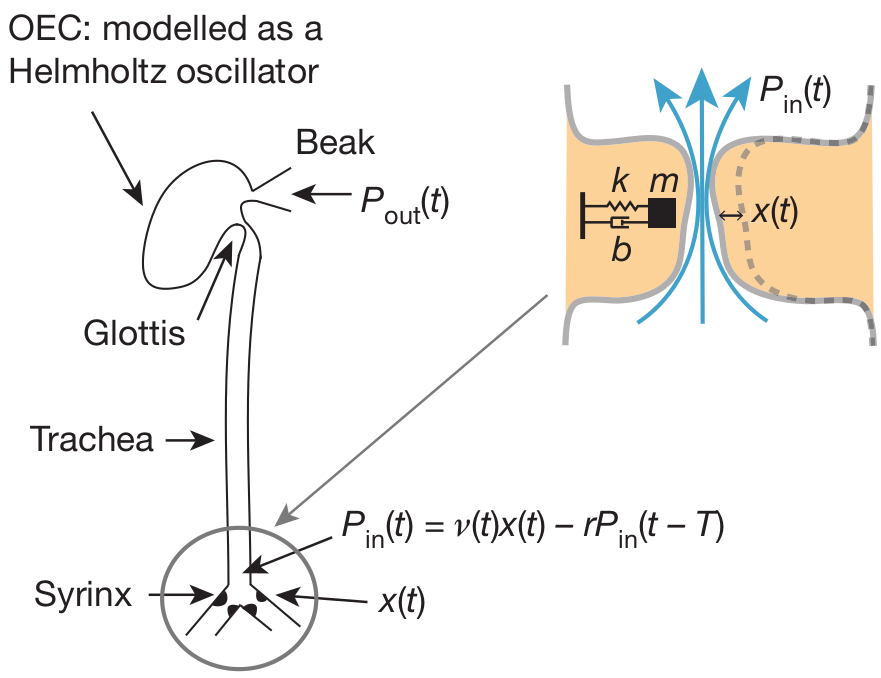
\includegraphics[width=0.5\linewidth]{media/scheme_vocal_apparatus}
  \caption{Model of the zebra finch vocal apparatus\label{zf-vocal-aparatus}}}
  \small

  The air (\(P_{sub}(t)\)) comes from the air sac below the syrinx, then goes up
  to the trachea, the glottis, resonate in the oro-esophageal cavity (OEC) and
  the beak (\(P_{out}(t)\)). Each component acts as a filter in G.B. Mindlin's
  team model of the zebra finch vocal aparatus. Figure 1b taken from
  \textcite{amador_elemental_2013}.

\end{figure}

G. B. Mindlin and his team built a model of the Zebra Finch vocal apparatus.
They described with differential equations the behaviour of the components of
this vocal apparatus (see Fig~\ref{zf-vocal-aparatus}). The differential
equations model the separation between the syringeal labia. Each labia are
modeled as a spring and mass system that can produce sustainable oscillations.
Depending of the parameters it receives, the synthesizer is able to produce a
vast variety of sounds, either very pure or very rough, depending of the
strength of the labia tension \parencite{amador_beyond_2008,
boari_automatic_2015}.

They simplified their model and obtained the dynamic system shown in equation
\ref{synth_eq_dyn}.

\begin{equation}
\systeme*{
\dv{x}{t} = y,
\dv{y}{t} = - \alpha \gamma^2 - \beta \gamma^2 x - \gamma^2 x^3 - \gamma x^2 y
    + \gamma^2 x^2 - \gamma x y
}
\label{synth_eq_dyn}
\end{equation}

\(x\) describes the position of the syringeal labia. \(\gamma\) is a constant
which takes into account values specific for the Zebra Finch vocal apparatus.
\(\alpha\) and \(\beta\) are unit-less time-dependant parameters. \(\alpha\) is
proportional to the air sac pressure, that is how much air is coming through the
syrinx, and \(\beta\) is proportional to the syringeal labial tension. It can be
hypothesized that these two parameters can be easily modified by motor actions.
Therefore, the whole singing behaviour can be described as the dynamics of
muscles acting on the air sac pressure and the syringeal labial tension. This
synthesizer provides thus a way to bridge the gap between actual motor commands
and song production. Even if the model is simplified, as it assumes a symmetry
in the labial tensions, it is able to produce a rich variety of sounds.
\textcite{amador_beyond_2008, perl_reconstruction_2011} studied the parameter
space and even showed that different categories of sound productions can be
found in different regions of the parameters space.

This model of birdsong production shows that low dimensional but biologically
realistics parameters can describe the singing behaviour. Simple variations in
the motor space produces complex and diverse variations in the song production.
This model simplifies greatly the study of song production behaviour, as it is
possible to study the dynamics of song production in the motor space while
keeping realistic constraints.

\subsection{Zebra Finches are sensible to song produced by the synthesizer}
\label{zebra-finches-are-sensible-to-song-produced-by-the-synthesizer}

The computational model of the zebra finch vocal apparatus is a real sound
synthesizer. It produces sound waves which birds, as we, can listen to. As
explained in \ref{neurobiology-of-the-zebra-finch}, Zebra Finches have neurons
which are highly selective to their BOS. When the bird is asleep and listen to
their own song, these neurons fire in a very specific pattern. To assess the
quality of their synthesizer, G.B. Mindlin team tested if their synthetical
song, built from the BOS, will activate these neurons
\parencite{amador_low_2014, boari_automatic_2015}. They showed that even if the
strenght of the activation was not as strong as the BOS, their synthesized song
performed better than a conspecific song or the BOS played in reverse. This
suggests that the synthesis is sufficiently good to trick a bird and therefore
a good imitation of its song.

\subsection{Gestures and song structure} \label{gestures-and-song-structure}

The study of the parameters \(\alpha\) and \(\beta\) over the time course of the
song reveals interesting results. \textcite{amador_elemental_2013} propose to
describe songs by the sequence of air sac pressure (\(\alpha\)) and syringeal
labial tension (\(\beta\)) trajectories, called gestures. A gesture starts and
stops when there is a discontinuity in the trajectory of either the air sac
pressure or the tension (see Fig~\ref{gestures_schema}). If notes and syllables
are the primitives of a song in the sensory space, a gesture is the primitives
of a song in the motor space. A syllable is most of the time generated by a
succession of several gestures. Amador and her collaborators suggested that
spiking pattern observed in HVC is correlated with the onset and offset of
gestures. It would have suggested that HVC activity is not a clock-like pattern
but the transmission of high level motor commands which defines the song
structure. This has been contested by \textcite{lynch_rhythmic_2016} and
\textcite{picardo_population-level_2016} with extensive statistical analyses.
Even if HVC neurons do not actually fire on the onset and offset of gestures,
the gesture framework is very interesting because it allows us to think about
the song structure representation in the motor space, and especially motor
discontinuities.

\begin{figure}[htbp]
  {\center
  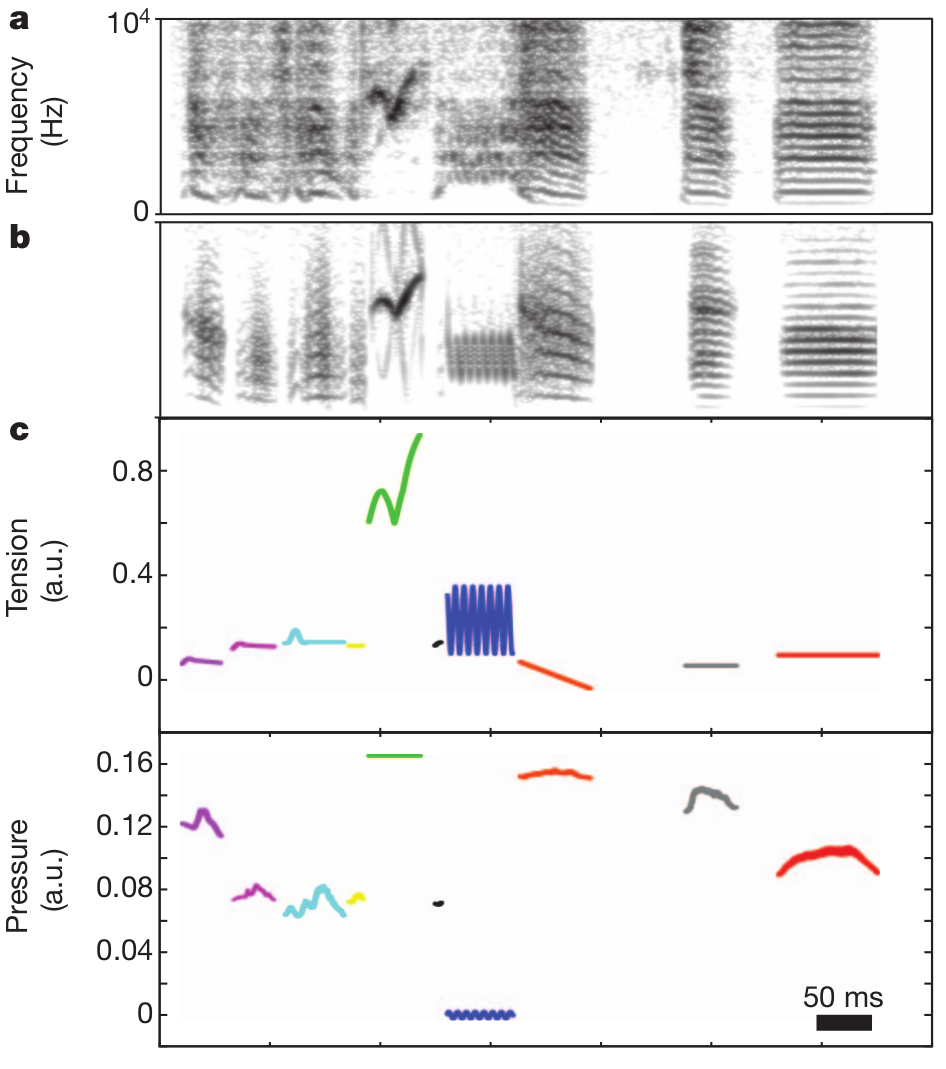
\includegraphics[width=0.5\linewidth]{media/gesture_schema_amador}
  \caption{A birdsong and its associated parameters for reproduction segmented
  in gestures\label{gestures_schema}}}

  \small
  \textbf{a)} spectrograph of a bird's song. \textbf{b)} spectrograph of the
  synthetic song. \textbf{c)} the paramaters \(\alpha\) and \(\beta\) for the
  song. There is several discontinuities in their trajectories. Each continuous
  segment forms a gesture. Figure from \textcite{amador_elemental_2013}.

\end{figure}

\section{Influence of Sleep in the Zebra Finch song development}
\label{influence-of-sleep-in-the-zebra-finch-song-development}

Several studies showed that sleep is involved in the song learning and
maintenance. \textcite{dave_song_2000} shows thanks to electrophysiology
recording the . \textcite{deregnaucourt_how_2005} showed that sleep has \todo{}

\subsection{Song replays during sleep}
\label{song-replays-sleep}

As explained in the Section~\ref{neurobiology-of-the-zebra-finch}, the song
system in the zebra finch brain is highly specialized. Neurons in HVC or RA have
a very precise and stereotyped pattern of activation when the adult bird sings.
\textcite{dave_song_2000} found surprising results. They recorded RA neurons
while adult birds were asleep. Neurons in RA spontaneously burst in patterns
similar to their activation patterns while the bird sing. Dave \& Margoliash
hypothesize that this replay activity could be the product of an off-line
learning mechanism. Indeed, neural replays have already been found in the rat
and it has been showed that these replays influence the construction of its cognitive maps \parencite{de_lavilleon_explicit_2015} or the suppression of the replays impairs the learning \parencite{girardeau_selective_2009}.

Dave \& Margoliash's results were obtained on adult birds which have already
learned their song. Though, we can hypothesize that RA replays also occur in the
juvenile bird and impacts its learning. The actual function of the mechanism
that produces these replays must still be determined.

\begin{figure}[tbph]
  {\center
  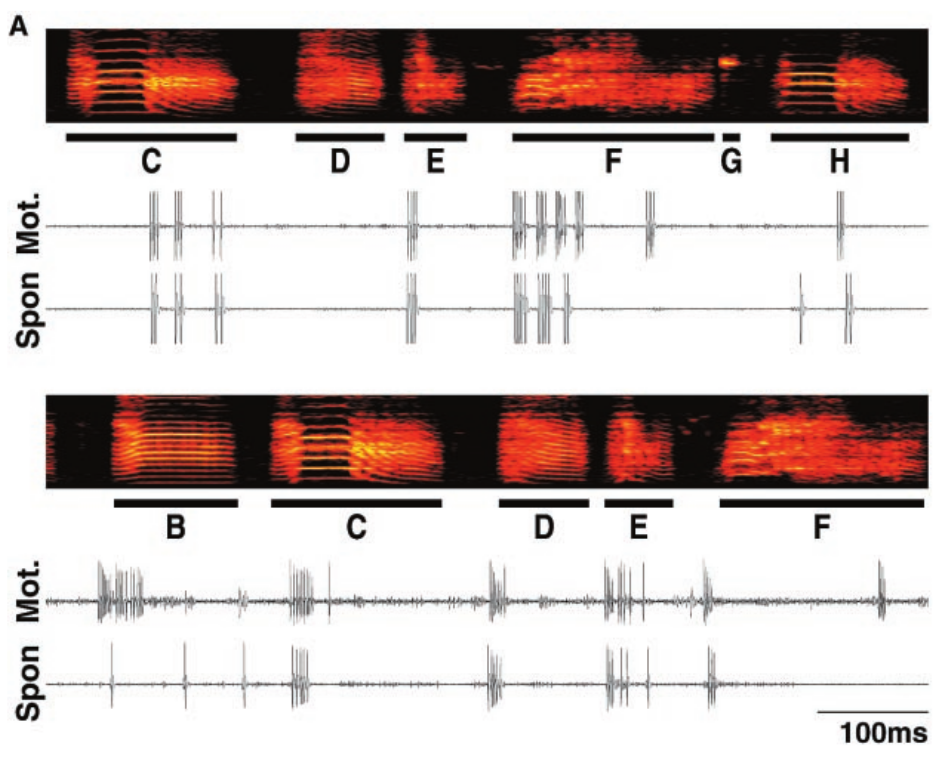
\includegraphics[width=0.7\linewidth]{media/replays_bird_margoliash}
  \caption{Neuronal replay during sleep}
  }
  \small
  Recording of trace of activity of two different neuron for one bird. For each
  neuron, a premotor activity is shown with the spectrograph of the song the
  bird sang and the raw trace of a spontaneous activity during sleep that
  matches the premotor pattern. Taken from \textcite{dave_song_2000}.

\end{figure}

\subsection{The impact of sleep on the birdsong learning}
\label{impact-sleep-birdsong-learning}

\textcite{deregnaucourt_how_2005} recorded entire song developments of Zebra
Finches and studied the vocal trajectories during the whole learning process as
during the cycles of sleep and wakefulness. They tracked the development of
syllables and clustered them. Thanks to this database, they computed the shift
in the mean of the clusters for each syllable either in the same day (2 random
samples of 100 songs), from evening to the morning (last 100 songs compared to
the first 100 songs of the next day) or from the middle of one day to the middle
of the next day (random sample of 100 songs compared to a random sample of 100
songs of the next day). They computed the total vocal change for each of these
cluster, that is the relative variation of syllable features
\textcite{tchernichovski_procedure_2000}\footnote{These measures are detailled
in Section~\ref{measures}}. They found
that vocal change was the most important with the comparison of the cluster of
the evening songs compared to the next day morning song, compared to the changes
that occur for one day to the next or in the same day (see
Fig~\ref{der_abs_vocal_change}). This result shows that sleep has a big impact
in the development of the birdsong, because it cannot be explained by the day to
day vocal change.

\begin{figure}[htpb]
  {\center
  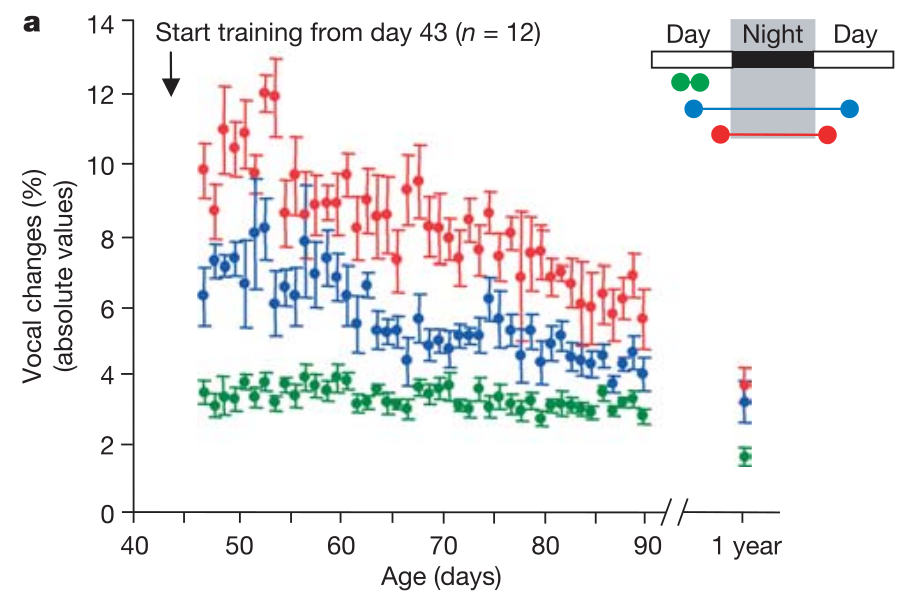
\includegraphics[width=0.7\linewidth]{media/der_absolute_vocal_change}
  \caption{Absolute vocal change during song development\label{der_abs_vocal_change}}}
  \small
  Vocal changes in absolute values (median + s.e.m). Green is the change across random sample during the same day (baseline). Blue is the change between random sample from one day to the next. Red is the vocal change from one evening to the next morning. Taken from \textcite{deregnaucourt_how_2005}.
\end{figure}

The vocal change measure Derégnaucourt and his team used is an absolute measure.
That means that this measure cannot tell if the change goes in the same trend as
the whole learning or in the opposite direction. Thus they introduce a signed
measure of vocal change. If the change goes in toward the value of the feature
at the end of the learning, the signed vocal change is positive, otherwise, it
is negative. The signed vocal change showed that sleep actually has a
\emph{negative impact} on learning. Indeed, the effect of night-sleep is almost
always negative (see Fig.~\ref{der_night_signed_change}). The effect cannot be
explained by the fact the bird has not sung for a long time. Indeed, preventing
the bird of singing for 8 hours does not yield the same effect. Thus, this
unlearning is due to a mechanism which occur during sleep.

\begin{figure}[htpb]
  {\center
  \subfloat[Vocal changes in signed values during sleep]{
    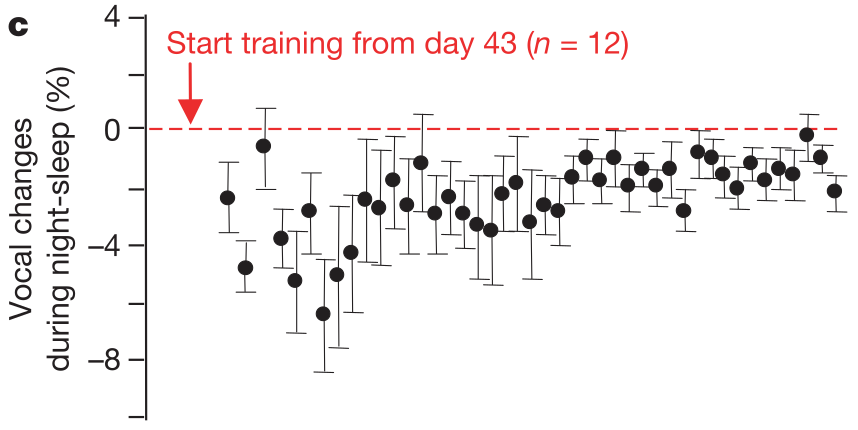
\includegraphics[height=5cm]{media/der_night_signed_change}
    \label{der_night_signed_change}
  }
  \subfloat[Entropy variance decreases during sleep]{
    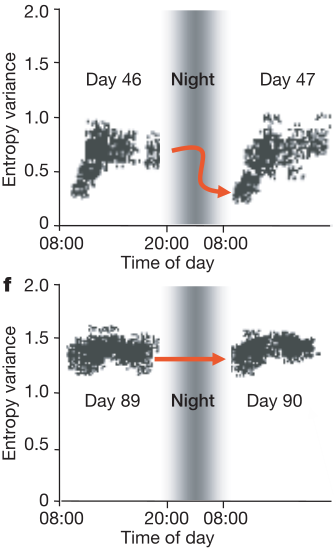
\includegraphics[height=7cm]{media/entropy_variance_night_effect}
    \label{entropy_var_night_effect}
  }
  }
  \caption{Sleep has a negative impact on vocal development}
  \small
  \textbf{a)} Vocal changes in signed values (median + s.e.m) during night-sleep compared to overall development trend.
  \textbf{b)} Entropy variance increase overall song development but decrease
  during night when the bird is still learning. At 90DPH, the bird has reach crystallisation of the song and sleep has little to no impact.
  Taken from \textcite{deregnaucourt_how_2005}.
\end{figure}

The authors computed the performance of the bird to reproduce its tutor song at
the end of its development thanks to a similarity measurement
\parencite[][developped in
section~\ref{measures}]{tchernichovski_procedure_2000}. Surprisingly, they found
that the more the post-sleep deterioration was important overall, the better the
bird was able to imitate the song of its tutor, as seen on
Fig.~\ref{der_sim_post_det}. The negative impact sleep has on learning on the
short term (day to day) has a positive impact in the long run. It shows that a
learning mechanism is at play during sleep. This learning mechanism has a
different function than the learning mechanism during the day. The author
suggest that the oscillations in vocal learning may help the bird get out of
local maxima in development. Several learning algorithm can be investigated to
explain these results.

\begin{figure}[htpb]
  {\center
  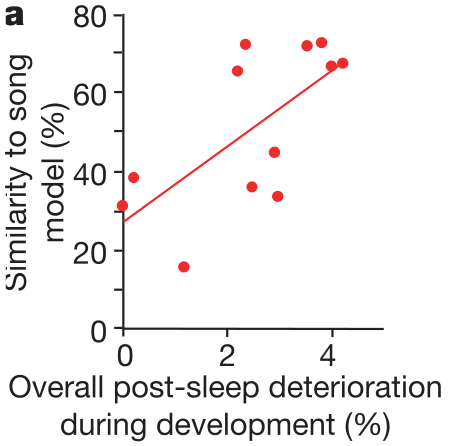
\includegraphics[width=0.3\linewidth]{media/cor_deterioration_sim}
  \caption{Correlation between post-sleep deterioration and similarity of the
  tutor song at the end of learning. \label{der_sim_post_det}}}
  \small
  The more the sleep deteriorate the bird's learning from one day to the next, the better the bird reproduces its tutor song at the end of its learning. Taken from \textcite{deregnaucourt_how_2005}.
\end{figure}


\section{A computational model of birdsong learning to explain the sleep
influence}
\label{a-computational-model-of-birdsong-learning-to-explain-the-sleep-influence}

\subsection{Interest of a computational model of birdsong learning}
\label{interest-of-a-computational-model-of-birdsong-learning}

  * Computational model helps understanding what are the \emph{implementation
  constraints} of the learning mechanisms
  * Use of synthesizer Realistic computational budget
  *Easily make hypotheses that can be tested experimentally afterwards
  Abstracted and controlled environment

\subsection{Goal: Build a modular two-step learning model and look for learning
algorithm that can account for Derégnaucourt's results.}
\label{goal-build-a-modular-two-step-learning-model}

\chapter{Our Model} \label{our-model}

The goal of this internship is to build a computational and behavioral model of
birdsong learning with realistic constraints and try to model the impact of
sleep on song development as presented in the
Section~\ref{impact-sleep-birdsong-learning}. The model is developped from
scratch in Python~3. It uses the birdsong synthesizer built by G.B.~Mindlin and
his team and the standard measures used to analyse birdsong.

The Model is a two-step learning model. The model alternates between two
different learning algorithm. The strong hypothesis we make is that one of these
learning algorithm correspond to the learning algorithm the bird uses during the
day, and  the second algorithm is the algorithm used by the bird during its
sleep. We hypothesize that the algorithm used during sleep should focus on
restructuration of the song models the bird has and to the diversity \todo{}. We
think that an algorithm targetting these \todo{} yields the negative impact of
sleep in the short term with a positive impact at the end of learning as
\textcite{deregnaucourt_how_2005} observed.

The source code of the model is available at
\url{https://github.com/PaulEcoffet/birdsonglearningmodel}.

\section{Global Architecture} \label{global-architecture}

The model is built in several modules. First of all, the model uses
G.B.~Mindlin's team synthesizer to produce realistic song with biologically
plausible parameters (see Section~\ref{song-synthesizer}). Then, song features
measurement and songs comparison methods have been implemented and used as the
hearing system. The song feature measures were taken from the litterature
\parencite{tchernichovski_procedure_2000}. They are the standard measures used
to describe songs and syllables in the birdsong research community.

As we are building a computational model, we had to explicit every aspect of the
song learning.

The birdsong learning model I built is a two step learning algorithm. One
algorithm models the learning process of the bird during the day, the other
models the learning during the night. These day and night models can be easily
changed in the program I wrote.

\subsection{Boari's implementation of the birdsong synthesizer}
\label{usage-of-boaris-implementation-of-the-birdsong-synthesizer}

We want to use G.B.~Mindlin's synthesizer because it allows us to build a
computational model with realistic constraints. It bridges the gap between the
motor command and the song production thanks to a biophysical model of the Zebra
Finch vocal apparatus. Our model can produce simple streams of \(\alpha\) and
\(\beta\) parameters and send it to the synthesizer. The synthesizer produces
real sound waves that can be analyzed by the hearing system.

We used the implementation of the synthesizer available for download on the
Dynamical System laboratory of the University of Buenos Aires
(\url{http://www.lsd.df.uba.ar}) \parencite{boari_automatic_2015}. The
downloaded program was actually a combination of a \(\alpha\) and \(\beta\)
parameter extractor from an audio file and the synthesizer from the extracted
parameters. I extracted the synthesizer from the source code and adapted it so
that it can receive arbitrary parameters. The synthesizer had several bugs. It
is suppose to generate a sound stream of the same length of the parameter
stream, that is, if there is 10~000 values of \(alpha\) and \(beta\) sampled at
44~100~Hz, the synthesizer should return a sound wave composed of 10~000 values
sampled at 44~100~Hz. But it actually dismiss 2 values, returning only 9~998
values. As the implementation of the synthesizer was badly documented and the
source code was not self explanatory at all, I decided to pad the \(\alpha\)
\(\beta\) streams with 2 dummy values to prevent this bug.

I have also developped a small Cython package to call Boari's C synthesizer from
Python. The source code of this package is available at
\url{https://github.com/PaulEcoffet/birdsynth}.

\subsection{Characterizing and comparing songs}

As we wanted to work on real audio signal, our algorithm must use relevant
features of the songs to describe them. Indeed, it needs to compare its
production to the tutor song so as to correct its errors and improve itself.

\subsubsection{Measurement of the song features}
\label{measures}
\textcite{tchernichovski_procedure_2000} suggested several measures to
characterize compare songs. To apply these measures, the song is first cut into
several time windows, and the measures are computed for each time windows. These
measures give us a fine-grained description of the song throughout time.
Tchernikovski and his colleague proposed also a measure of similarity between
two songs.

They are extensively used in the birdsong research community
\parencite{coen_learning_2007, deregnaucourt_how_2005, lipkind_stepwise_2013,
liu_juvenile_2004}.

The measure we used are the Amplitude, the Frequency Modulation, the Amplitude
Modulation, the Pitch, the Goodness and the Wiener Entropy of the signal.
Tchernikovski and his team developped a software called Sound Analysis Pro 2011
to compute these features. Though, this software runs only on Windows and its
function cannot be called by another program. I have thus ported the
implementation of the song features measurement from a Matlab implementation
(called Sound Analysis Toolbox) to a Python implementation. The values of the
features for the same song computed by my implementation matched qualitatively
the values of the Matlab implementation (see Figure~\ref{bsa_sat_match}).

I have also reimplemented the spectral derivative plot which is
extensively used in the songbird research community to represent songs.

\todo{insert graph to show the match}

\subsubsection{Comparison of two songs}

\textcite{tchernichovski_procedure_2000} introduced also a similarity
measurement. This similarity measurement compares how a song is related to its
tutor song. To do so, the algorithm of similarity measurement look for matches
in the features for each sound window of the tutor song and the pupil song. The
similarity score is the percentage of the tutor song that has been matched to
the pupil song. The similarity score does not punish wrong order of syllables.
For instance, if the pupil sings the syllables A-C-B instead of A-B-C, the
similarity will be very high even if the syllables are sung in the wrong order.

Similarity is really long to compute and is only meaningful when comparing two
complete songs. It is also almost unaffected by temporal mismatches.Other
methods are used to compare syllables or notes. For simplicity, syllables are
compared by the study of means and variance of every features (Pitch, Entropy,
\ldots{}) during the syllables. Two syllables are considered similar if they
have the same mean and variance for every features.

The Python module I wrote to compute song features and similarity scores is
called \emph{birdsonganalysis} and is available for download at
\url{https://github.com/PaulEcoffet/birdsonganalysis/}.

\subsection{Song Model}\label{song-model}



\subsubsection{Gesture paradigm inherited from
synthesizer}\label{gesture-paradigm-inherited-from-synthesizer}

\subsubsection{Gesture sequence}\label{song-structure}

  * List of gestures and their duration
  * Fixed duration of the song because of measurement

\subsubsection{Gesture composed of two generators for the motor
commands}\label{gesture-composed-of-two-generators-for-the-motor-commands}

  * Abstracted in sum of sin \& linear func

\subsection{Two-step learning model} \label{two-step-learning-model}

Our model is divided in two different phases.

  * Bird has several song models it trains to reach tutor
  * tutor song is known
  * day algorithm for parameters optimisation
  * night algorithm for structure optimisation
  * Hypothesis:~structure optimisation yield unlearning short term, better
  learning long term


\section{Day learning algorithm}\label{day-learning-algorithm}

\subsection{Goal}\label{goal}
  * Optimise gestures parameters
\subsection{Hillclimbing}\label{hillclimbing}

  * really simple
  * Choose song model, choose gesture
  * Choose close parameters, if better keep, if worse trash
  * Knows if better by comparison of weighted standard measurements
  * Not whole song but only gesture trained to make faster computations
        * Actually creates unlearning

  \subsection{Prediction}\label{prediction}
  * Should improve song production but get stuck in local maximum because
  bad structure
\section{Night learning algorithms}\label{night-learning-algorithms}

\subsection{Goal}\label{goal-1}

  * Find better structure to describe song motor command
\subsection{Several variations of algorithm have been
tested}\label{several-variations-of-algorithm-have-been-tested}

  * Evolutionary algorithm

        * Simple solution for structure variation
    * with or without diversity
\subsection{Algorithm}\label{algorithm}

  * Evolutionary algorithm Microbial GA
  * Increase population size and add variation in structure

        * Remove, add, change, copy gesture
      * Song always the same length for comparison reasons.
    * Compare by tournament
        * The winner put a variation of itself in place of the loser
        * Compare number of neighbour, score, lower the better
\subsection{Predictions}\label{predictions}

  * Structure variation yields unlearning short term but positive impact
  long term
  * Diversity will increase this

\section{Parameters}\label{parameters}

  * Tried to be realistic
  * most are fit through gridsearch
  * Realistics: Number of days, number of syllables sung during all dev
  * Gridsearch optimisation
  * Default value for gesture parameters
  * Learning rate
        * Prevent part of unlearing
      * Could be fitted to match real song learning rate
      * Coefficient for score optimisation
    * Algorithm way better in score than Boari but qualitatively very
  different to the ear
  * Look at which parameters boari's method was better than algo and put
  priority on them
  * Amplitude and entropy
  * Diversity threshold to maximise variance in diversity score

        * Value: 5000
      * Other parameters
    * Number of song models during day and night: Depend of runs
  * Boundaries for parameters values: Fixed
  * Number of tournaments during night: depend of runs
        * Correlated with replay? By how much?

\chapter{Analyses and results}\label{analyses-and-results}

\section{Learning method is as good Boari's method or
better}\label{learning-method-is-as-good-boaris-method-or-better}

  * Using standard measure criteria in the birdsong community
  * Simple description of motor params sufficient to produce good songs
  * Qualitatively same amount of gestures
        * Can be due to luck

  \section{Too little training per model cause
divergence}\label{too-little-training-per-model-cause-divergence}

  * maybe due to global vs local error
\section{Derégnaucourt results not
reproduced}\label{deruxe9gnaucourt-results-not-reproduced}

  * Syllables extracted by time of begin and end
  * Without or with diversity
  * No night deterioration
  * Night deterioration has no impact in overall learning
\chapter{Discussion}\label{discussion}

\section{The synthesizer which cannot produce every
sounds}\label{the-synthesizer-which-cannot-produce-every-sounds}

  * Our score really close to boari's method (not way better or way
  worst), maybe we reached synthesizer limits
\section{The parameters description we
choose}\label{the-parameters-description-we-choose}

  * more simple/complexe possible than sum of sin and affine?
\section{The unlearning during day due to the gesture
learning}\label{the-unlearning-during-day-due-to-the-gesture-learning}

\section{Fixed duration of songs in
learning}\label{fixed-duration-of-songs-in-learning}

  * Dynamic Time Warping can correct that
\section{Big artificial separation between structuration and gestures
optimisation}\label{big-artificial-separation-between-structuration-and-gestures-optimisation}

\section{Diversity not strong enough? What if only diversity during
night?}\label{diversity-not-strong-enough-what-if-only-diversity-during-night}

  * Maybe not convergence
  * Maybe what we are looking for
\chapter{Conclusion}\label{conclusion}

\section{Learning algorithm with two step
learning}\label{learning-algorithm-with-two-step-learning}

  * Very few of them
  * Working with realistic synthesizer
  * modular architecture, easy to test new models
\section{Restructuration didn't yield the expected
effect}\label{restructuration-didnt-yield-the-expected-effect}

 * More parameters search might be able to fix it

\printbibliography{}

\end{document}
